\section{Diagramas de Penrose y estructura causal.}
la idea detrás de los diagramas espacio-tiempo  de Penrose es representar la estructura causal de un espacio-tiempo en un diagrama bidimensional finito, mediante una compactación conforme , estos muestran la propagación de señales y partículas en el espacio-tiempo.

En un diagrama de Penrose, el espacio-tiempo se representa en un plano bidimensional, donde el eje vertical representa el tiempo y el eje horizontal representa el espacio. En esta representación se mantienen los conos de luz formando un angulo de $45$ grados . Las líneas horizontales y verticales representan  tiempo constante y espacio constante respectivamente .


Con el propósito de construir los diagramas de Penrose, podemos seguir la siguiente receta,
(Es una receta en términos de que no hay un algoritmo perfectamente delimitado, siempre nosotros debemos de agregar algo mas )


\begin{enumerate}
    \item Empieza con alguna métrica en algún sistema de coordenadas no compacto (nota el rango de las coordenadas)
    \item Encuentra una coordenadas tales que las anteriores sean reemplazadas por coordenadas nulas
    \item Compacta las dos coordenadas nulas de forma separada
          Para esto hay varias maneras y varias funciones que cumplen este requisito, por ejemplo $sinh(x)$ o $tanh(x)$ o $tan^{-1}(x)$, cada una de estas son funciones biyectivas de los reales $\mathbb{R} $ a un dominio compacto.


          En este caso se introduce las nuevas coordenadas como:
          \begin{equation}
              \begin{array}{l}
                  p:=\tan ^{-1}(v) \\
                  q:=\tan ^{-1}(w)
              \end{array}
          \end{equation}
          Donde el par ordenado $(p,q)$ tomara valores dentro de un subconjunto de rango
          $(\frac{-\pi}{2},\frac{\pi}{2})X(\frac{-\pi}{2},\frac{\pi}{2})$
          (La elección  de la función tangente inversa es arbitraria, pero es una elección común, para el caso de Minkowski es posible también hacer  esta compactación con la función $sinh(x)$)
    \item Define de nuevo coordenadas espaciales y temporales
          \begin{equation}
              \begin{array}{l}
                  T:=p+q \\
                  X:=p-q
              \end{array}
          \end{equation}
          (Mantén una "bitácora" de los rangos de estas coordenadas, ya que la información de esta transformación esta dada por donde se encuentran las nuevas fronteras finitas)
\end{enumerate}
\subsection{Diagrama en el espacio-tiempo de Minkowski}
El espacio-tiempo de Minkowski es la solución mas sencilla de las ecuaciones de campo, donde las coordenadas poseen los rangos:
\begin{equation}
    \begin{array}{c|c|c|c}
        t                  & r           & \theta   & \varphi   \\
        ( -\infty, \infty) & (0, \infty) & (0, \pi) & (0, 2\pi)
    \end{array}
\end{equation}
y la métrica es:
\begin{equation}
    ds^2 = -dt^2 + dr^2 + r^2 d\Omega^2,
\end{equation}
nótese  que se expreso en unidades naturales donde $c=1$.
Definimos las coordenadas nulas $v$ y $w$ como:
$$
    \begin{array}{ll}
        v:=t+r & r = \frac{1}{2}(v-w) \\
        w:=t-r & t = \frac{1}{2}(v+w)
    \end{array}
$$
Donde los rangos de las nuevas coordenadas son  $r=\frac{1}{2}(v-w)>0 \longrightarrow v>w$.
Las coordenadas nulas $v$ y $w$ son compactificadas con la función tangente inversa, obteniendo las coordenadas $p$ y $q$:
$$ p:=\tan ^{-1}(v) \\
    q =\tan ^{-1}(w)
$$
Debido a que la función tangente inversa es monótona creciente, se tiene que $v>w \longrightarrow p>q$ y cambia el rango del par ordenado $v,w \in (-\infty, \infty) \longrightarrow p,q \in \left(-\frac{\pi}{2}, \frac{\pi}{2}\right)$.

Una vez que las coordenadas nulas han sido compactificadas, se definen las coordenadas temporales y espaciales $T$ y $X$ como:
$$
    \begin{array}{ll}
        T:=p+q, & p = \frac{1}{2} (T + X) \\
        X:=p-q, & q = \frac{1}{2} (T - X)
    \end{array}
$$
y los nuevos rangos de estas coordenadas son:

\begin{equation}
    \left[\begin{array}{c}
            -\frac{\pi}{2}<\frac{1}{2}(T+X)<\frac{\pi}{2} \\
            -\frac{\pi}{2}<\frac{1}{2}(T-X)<\frac{\pi}{2} \\
            \frac{1}{2}(T+X)>\frac{1}{2}(T-X)
        \end{array}\right] \Leftrightarrow\left[\begin{array}{l}
            -\pi<T+X<\pi \\
            -\pi<T-X<\pi \\
            X>0
        \end{array}\right]
\end{equation}
por lo ahora podemos dibujar la región permitida
\begin{figure}[H]
    \centering
    \shorthandoff{>}
    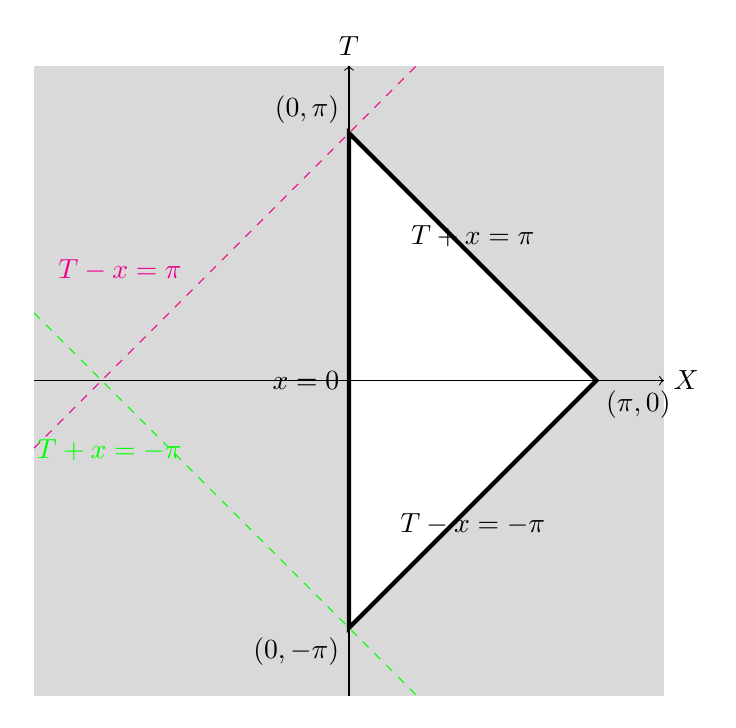
\begin{tikzpicture}[scale=1]

        % Definimos la constante pi
        \pgfmathsetmacro{\mypi}{3.1416}

        % Fondo gris para toda el área de dibujo (ajustable)
        \fill[gray!30] (-4,-4) rectangle (4,4);

        % Región permitida (blanca): para x>0, T entre -pi+x y pi-x
        \fill[white] (0,-\mypi) -- (0,\mypi) -- (\mypi,0) -- cycle;

        % Límites sólidos de la región permitida:
        % T+x=\pi  =>  T=\pi-x, que une (0,\pi) con (\mypi,0)
        % T-x=-\pi =>  T=-\pi+x, que une (0,-\mypi) con (\mypi,0)
        % y la recta x=0 (eje vertical) que une (0,-\mypi) con (0,\mypi)
        \draw[line width=1.5pt] (0,-\mypi) -- (0,\mypi) -- (\mypi,0) -- cycle;

        % Límites adicionales (discontinuos) de las otras inecuaciones:
        % 1. T+x=-\pi  =>  T=-\pi-x (línea discontinua en verde)
        % Se dibuja en un rango amplio de x para visualizarla.
        \draw[dashed,green] (-4, {4 - \mypi}) -- (0.9, {-0.9 - \mypi});

        % 2. T-x=\pi   =>  T=\pi+x (línea discontinua en magenta)
        \draw[dashed,magenta] (-4, { \mypi - 4 }) -- (0.9, { \mypi + 0.9 });

        % Etiquetas para los límites (se pueden ajustar las posiciones):
        % Etiqueta de la frontera T+x=\pi (límite sólido superior de la región)
        \node[above, black] at ({0.5*\mypi}, {0.5*\mypi}) {$T+x=\pi$};

        % Etiqueta de la frontera T-x=-\pi (límite sólido inferior de la región)
        \node[below, black] at ({0.5*\mypi}, {-0.5*\mypi}) {$T-x=-\pi$};

        % Etiqueta para la frontera T+x=-\pi (línea discontinua, verde)
        % Se coloca en un punto representativo, por ejemplo, en x=-2.
        \node[above left, green] at (-2, { -\mypi + 2 }) {$T+x=-\pi$};

        % Etiqueta para la frontera T-x=\pi (línea discontinua, magenta)
        \node[above left, magenta] at (-2, { \mypi - 2 }) {$T-x=\pi$};

        % Etiqueta para la frontera x=0 (eje vertical)
        \node[left] at (0,0) {$x=0$};

        % Se dibujan los ejes coordenados
        \draw[->] (-4,0) -- (4,0) node[right] {$X$};
        \draw[->] (0,-4) -- (0,4) node[above] {$T$};

        % Etiquetas de los vértices de la región permitida
        \node[below left] at (0,-\mypi) {$(0,-\pi)$};
        \node[above left] at (0,\mypi) {$(0,\pi)$};
        \node[below right] at (\mypi,0) {$(\pi,0)$};

    \end{tikzpicture}
    \caption{Regiones definidas por \(-\pi<T+x<\pi\), \(-\pi<T-x<\pi\) y \(x>0\). Límites sólidos: región permitida (\(T+x=\pi\) y \(T-x=-\pi\)); discontinuos: fronteras de las inecuaciones restantes.}
\end{figure}

para el caso de Minkowski, la región permitida es un rombo, donde las líneas diagonales representan la luz, las líneas horizontales representan el espacio constante y las líneas verticales representan el tiempo constante.





%%%%%%%%%%%%%%%%%%%%%%%%%%%%%%%%%%%%%%%%%%%%%%%%%%%%%%%%%%%%%%%%
%   % material extra no se si agregarlo
%   \item \textbf{Transformación conforme en diagramas de Penrose:} Para construir el diagrama de Penrose, utilizamos una transformación conforme que reescala la métrica para compactificar el espacio-tiempo. La métrica en coordenadas $(T,X,\theta,\varphi)$ se expresa como:
%   \begin{equation}
%       g = \Omega^{-2}(T,X,\ldots)\left(dT\otimes dT - dX\otimes dX - R(T,X)[\text{términos angulares}]\right).
%   \end{equation}
%   El factor conforme $\Omega^{-2}$ aparece multiplicando toda la métrica. Definimos una nueva métrica (no física) multiplicando por $\Omega^2$:
%   \begin{equation}
%       g_{\text{diagram}} = \Omega^2 g.
%   \end{equation}
%   Sustituyendo la expresión de $g$ en la ecuación anterior, obtenemos:
%   \begin{equation}
%       g_{\text{diagram}} = \Omega^2 \times \Omega^{-2} \left( dT\otimes dT - dX\otimes dX - R(T,X)[\text{términos angulares}] \right).
%   \end{equation}
%   Como $\Omega^2 \times \Omega^{-2} = 1$, el factor conforme se cancela, dejando:
%   \begin{equation}
%       g_{\text{diagram}} = dT\otimes dT - dX\otimes dX - R(T,X)[\text{términos angulares}].
%   \end{equation}
%   Nos interesa principalmente la estructura causal, la cual está contenida en la parte $(T,X)$ de la métrica. Por lo tanto, suprimiendo los términos angulares, obtenemos:
%   \begin{equation}
%       g_{\text{diagram}} = dT\otimes dT - dX\otimes dX.
%   \end{equation}
%   La elección del factor conforme $\Omega$ y de las nuevas coordenadas $(T,X)$ se hace de manera que el infinito de la métrica original se mapea a puntos finitos en el diagrama. Esto permite representar todo el espacio-tiempo en una región compacta, facilitando el análisis de su estructura causal.
%   

%   Remarks: (1) One chooses, in tep (ii), null coords, and compactifies these in step (iii), because these preserve the causal structure.
%   (2) Max owr, dropping the conformal factor $\Omega^{-2} \neq 0$ does afect the shape of timelike and spacelike geodesics but not of null geodesics

%   More precisley:
%   $\gamma$ is a null geodesic of a metric $g$ iff
%   $\gamma$ is a mull geodesic  of the metric $\Omega^2 g$, Whre $\Omega^2$ is a nowhere vanishing smoth function on the manifold. proof $\rightarrow$ Tutonals.